\chapter{Redes Neurais} \label{cap:neurais}

Neste capítulo introduziremos redes neurais como uma forma genérica para escrever famílias de funções. Os conceitos de composição, tipos de camadas e arquiteturas são introduzidos. Daremos um enfoque aos dois tipos de camadas que foram usados no presente trabalho. Posteriormente, detalhes técnicos do treino de redes neurais são explorados. Por fim, apresentamos trabalhos selecionados da literatura que utilizaram redes neurais para a quebra de CAPTCHAs de texto.

\section{Introdução}

Dentro do campo de Inteligência Artificial, aprendizado de máquina é uma abordagem algorítmica para inferir regras em um problema a partir de exemplos. Uma categoria especial é a de aprendizado supervisionado, onde os exemplos constituem-se de um \textit{elemento} em um domínio conhecido e um \textit{rótulo} associado. O objetivo é deduzir abstrações que permitam relacionar elementos e rótulos. Nesse contexto, uma rede neural\footnote{Apesar de introduzidas aqui como um algoritmo supervisionado, redes neurais podem ser aplicadas de forma efetiva à problemas não supervisionados.} é, em última análise, uma forma genérica de escrever funções\footnote{Funções estão sendo usadas aqui com um sentido mais relaxado do que o usualmente utilizado na matemática.} sobre relações elemento-rótulo. Dada uma métrica para a estimativa dos erros cometidos por uma relação inferida, o desafio de inferir regras de associação ótimas se torna um problema de encontrar uma função que minimiza nossa estimativa de erro. O adjetivo '\textit{neural}' advém da inspiração em funções biológicas que historicamente influenciaram e ainda influenciam essa forma de exprimir relações. Em resumo, redes neurais são um conjunto de técnicas inspiradas em processos cognitivos desempenhados pelo sistema nervoso que fornecem uma maneira genérica de descrever famílias de funções.

De forma mais específica, dado um conjunto de exemplos $D = \{(x, y)\}$, onde $x$  pertence algum domínio conhecido e $y$ um rótulo associado, desejamos encontrar a função $\hat{y} = f(x)$, de tal modo que $\hat{y}$ seja o mais similar possível à $y$. Por '\textit{mais similar o possível}' entende-se que conhecemos uma estimativa para os erros, também referida como função custo, que é tão menor quanto melhor for a aproximação dada por $f(x)$, e é normalmente representada como $J(y, \hat{y})$. Formalmente, desejamos encontrar $f^*$ tal que
\begin{equation}
f^* = \argmin_{\{f\}} J^{(D)} = \argmin_{\{f\}} \langle J(y, f(x)) \rangle_{D},
\end{equation}   
onde $\langle \ldots \rangle_{D}$ representa o valor esperado no conjunto $D$.

Dada uma família de funções $f^{\mathbf{\Theta}} : x \rightarrow y$ definida por uma rede neural e parametrizadas por $\mathbf{\Theta}$, podemos vasculhar o espaço de busca induzido, $\{\mathbf{\Theta}\}$, para encontrar um função que satisfaça alguma propriedade de interesse. Em particular, no caso de aprendizado de máquina, estamos interessados em encontrar o parâmetro $\mathbf{\Theta}^*$ tal que:
\begin{equation}\label{thetaotimo}
\mathbf{\Theta}^* = \argmin_{\{\mathbf{\Theta}\}} \langle J(y, f^{\mathbf{\Theta}}(x)) \rangle_{D}.
\end{equation} 

A versatilidade desse formalismo nos permite explorar diferentes tipos de estruturas relacionais. Em particular, relações hierárquicas podem ser emuladas utilizando-se composição de funções. Essa abordagem nos permite construir redes neurais mais complexas e expressivas a partir de unidades básicas mais simples. Neste caso, podemos reescrever a função $f^{\mathbf{\Theta}}$ como:
\begin{equation}\label{fcamadas}
f^{\mathbf{\Theta}}(x) = f_1^{\mathbf{\Theta}^{(1)}}(f_2^{\mathbf{\Theta}^{(2)}} (f_3^{\mathbf{\Theta}^{(3)}}(\ldots(x))) ),
\end{equation}
sendo $\mathbf{\Theta} = (\mathbf{\Theta}^{(1)}, \mathbf{\Theta}^{(2)}, \mathbf{\Theta}^{(3)}, \ldots)$ o parâmetro composto por cada um dos parâmetros individuais.
Quando compomos funções desta forma, é comum nos referirmos à cada função $f_i^{\mathbf{\Theta}^{(i)}}$ como sendo a $i$-\textit{ésima} \textit{camada} da rede neural, sendo as camadas para além da mais externa também conhecidas como \textit{camadas escondias} (em inglês \textit{hidden layers}). A \textit{profundidade} da rede é uma referência à quantidade de funções internas usadas na composição. Diferentes tipos de funções definem diferentes tipos de transformações, as quais nos referimos como \textit{tipo da camada}. A especificação de todas as camadas em uma rede neural é o que chamamos de \textit{arquitetura} da rede. Não existe um consenso sobre o que seria exatamente a profundidade de uma arquitetura, ou a partir de que ponto podemos chamá-la de profunda \cite{Goodfellow-et-al-2016}. Neste trabalho vamos adotar a convenção de que a profundidade de um modelo é dado pelo número de camadas e que uma arquitetura é profunda se possuir mais de uma camada escondida. A seguir vamos explorar dois tipos de camadas que foram utilizados no presente estudo.

\section{Camadas Densas}

Camadas \textit{densas} ou totalmente conectadas definem uma transformação afim entre o conjunto de entradas e saídas. Tipicamente, após a transformação afim, segue-se a aplicação de uma função não linear elemento-à-elemento, conhecida como \textit{função de ativação}, permitindo a expressão de relações mais complexas. As camadas densas são biologicamente inspiradas no mecanismo de comunicação dos neurônios, onde a diferença de potencial elétrico exprimida nas sinapses do axônio é proporcional, em alguma medida, à soma das diferenças de potenciais experimentadas nos dendritos \cite{GerstnerNeuronalDynamics}. As conexões de entrada em um neurônio e sua regra de composição dos sinais definem sua regra de ativação, ou seja, quais outros neurônios devem estar ativos (e em que intensidade) para que haja uma transição de estado. Como veremos mais adiante, camadas totalmente conectadas tentam emular o comportamento de vários neurônios simultaneamente.

De maneira mais formal, seja $\mathbf{x}$ um vetor no conjunto de entrada, a relação expressa por uma camada densa é dada por:
\begin{equation}\label{denseop}
f^{\mathbf{W},\mathbf{b}}(\mathbf{x}) = act(\mathbf{W} \cdot \mathbf{x} + \mathbf{b})
\end{equation}
onde $\mathbf{b}$ é referido como \textit{viés} (ou, no inglês, \textit{bias}), $\mathbf{W}$ uma matriz de transformação, $act$ uma função de ativação e $\cdot$ é a operação usual de multiplicação de matrizes, definida elemento-à-elemento como $[\mathbf{W} \cdot \mathbf{x}]_{i} = \sum_k W_{ik} x_k$. Diferentes funções de ativação expressam relações distintas sob um vetor de entrada $\mathbf{z}$. Dentre os exemplos mais conhecidos na literatura, ressaltamos a função sigmoide, $\sigma(\mathbf{z})_i = \frac{1}{1+\exp(-z_i)}$, que mapeia os elementos de saída no intervalo $\Re[0,1]$, a função de retificação linear (relu), $relu(\mathbf{z})_i = max(0, z_i)$, e a função máximo atenuado (softmax), $\sigma(\mathbf{z})_i = \frac{\exp(z_i)}{\sum_j \exp(z_j)}$, que possui a interessante propriedade $\sum_i \sigma(\mathbf{z})_i = 1$, sendo usualmente utilizada para expressar distribuições de probabilidade.

Podemos interpretar a transformação expressa na equação \ref{denseop} como uma projeção do exemplo $\mathbf{x}$ sob um espaço de características que descrevem uma relação que desejamos expressar. De fato, se reescrevermos a $i$-\textit{ésima} linha de $\mathbf{W}$ como $\alpha_i \hat{\mathbf{w}_i}$, onde $\hat{\mathbf{w}_i}$ é um vetor normalizado e $\alpha_i$ a constante de normalização, podemos interpretar cada uma das saídas de uma camada densa (antes da função de ativação) como uma série de projeções balanceadas $\alpha_i \hat{\mathbf{w}_i} \cdot \mathbf{x} + b_i$ ($\cdot$ aqui é o produto interno usual). Em outras palavras, a contribuição da $i$-\textit{ésima} saída da camada é dada pela importância $\alpha_i$ dessa característica multiplicada por o quanto do exemplo é composto por essa característica,  $\hat{\mathbf{w}_i} \cdot \mathbf{x}$, adicionado de um viés $b_i$ que independe do exemplo em questão. Assim, para camadas densas, determinar os parâmetros ótimos pode ser entendido como encontrar projeções do espaço de entrada em um conjunto de características que sejam pertinentes ao problema. Neste sentido, cada saída de uma camada densa pode ser interpretada como um neurônio, que exprime em sua saída uma soma ponderada dos estímulos de entrada. Quando compomos camadas densas expressamos características que dependem de outras características. Durante o aprendizado, esperamos que essas projeções sejam descobertas de forma automática pelo modelo. Um desenho esquemático de como essas projeções funcionam pode ser visto na figura \ref{conv_lin}. O número de parâmetros em uma camada densa é dado pelo produto entre tamanho do exemplo de entrada e a quantidade de características.

\begin{figure}[ht!]
	\caption{Imagem ilustrativa das possíveis projeções aprendidas em uma camada (a) densa e (b) convolucional em um problema de reconhecimento de faces.}
	\begin{center}
	\begin{subfigure}{0.6\textwidth}
		\centering
		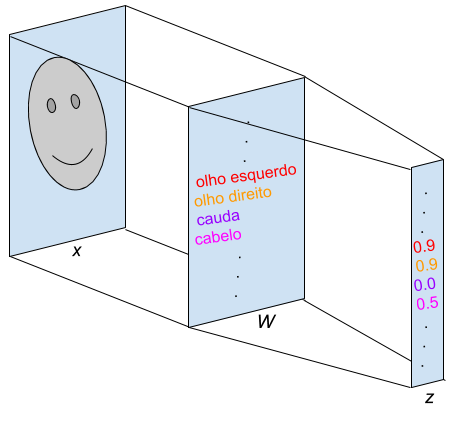
\includegraphics[width=.85\linewidth]{figuras/projlin.png}
		\caption{}
	\end{subfigure}%
	\vspace{.05\linewidth}
	\begin{subfigure}{0.6\textwidth}
		\centering
		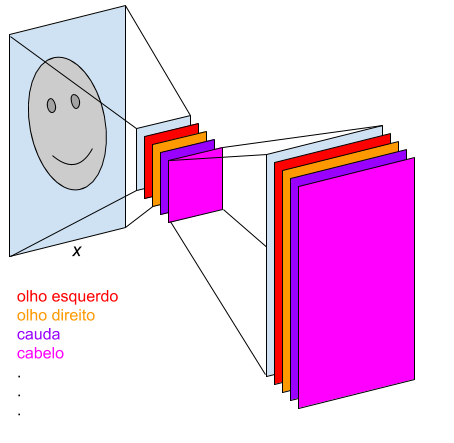
\includegraphics[width=.85\linewidth]{figuras/projcon.png}
		\caption{}
	\end{subfigure}
	\end{center}
	\small Em (a) as projeções atuam sobre todo o exemplo de entrada, mapeando-os em um espaço de importâncias de cada característica. Note que as projeções densas são fixas, no sentido que expressamos '\textit{olho direito}' em uma posição específica. Em (b) expressamos projeções menores que '\textit{varrem}' o exemplo de entrada buscando por uma característica em particular, projetando o exemplo em canais de características. Note que, neste caso, procuramos por uma característica que esteja presente em qualquer lugar da imagem, com os sinais de resposta registrados no canal respectivo. (Fonte: elaborado pelo autor.)
	\label{conv_lin}
\end{figure}

\section{Camadas Convolucionais}

Camadas \textit{convolucionais} \cite{LeCun1989, LeCun98} possuem similares com as densas: definem uma transformação afim representada por uma matriz, seguida, possivelmente, de uma função de ativação. Diferem, entretanto, no tipo de operação matricial utilizada, trocando-se o produto usual de matrizes por uma operação convolucional. Como vimos na seção anterior, as saídas de uma camada densa podem ser interpretadas como uma coleção de projeções independentes do exemplo de entrada sob um espaço de características. Em camadas convolucionais, o mesmo operador projeção é reutilizado em diferentes subespaços do conjunto de domínio, varrendo o mesmo exemplo em busca de padrões específicos em diferentes localizações. Esta peculiaridade é usualmente referida como \textit{compartilhamento de parâmetros}. O reuso promove a vantagem de reduzir consideravelmente o espaço de busca $\{\mathbf{\Theta}\}$ (Uma imagem ilustrativa do funcionamento dessas camadas pode ser visto na figura \ref{conv_lin}). O número de parâmetros nesse caso é dado pelo produto entre o tamanho da projeção e o número características. Camadas convolucionais são especialmente efetivas quando os elementos do domínio possuem alta localidade, como é o caso de imagens (cada pixel é altamente correlacionado com seus vizinhos em imagens naturais) e séries temporais periódicas (o valor da série do tempo $t$ é correlacionado com o valor da série em $t + \tau$, onde $\tau$ é o período da série). Tipicamente, mais de uma projeção é encapsulada em um mesmo tensor de transformação, sendo a matriz de cada projeção referida como núcleo. O resultado da convolução do núcleo com o exemplo de entrada é tipicamente referida como \textit{canal}.

Matematicamente, dado um tensor $\mathbf{x}$, a atuação da camada de convolução pode ser escrita como:
\begin{equation}
f^{\mathbf{W}, \mathbf{b}}(x) = act(\mathbf{W} \otimes \mathbf{x} + \mathbf{b})
\end{equation}
onde $\mathbf{W}$ é um tensor de transformação que encapsula a informação de diferentes projeções, $\mathbf{b}$ é o vetor de viés, de dimensão igual ao número de canais de saída, $act$ uma função de ativação e $\otimes$ é a operação de convolução, definida elemento-à-elemento por\footnote{Por simplicidade, estamos definindo aqui a operação de convolução para imagens coloridas, representadas por tensores de ranque $3$. Entretanto, operações de convolução podem ser definidas para outros domínios, como séries temporais (ranque $1$), imagens em tons de cinza (ranque $2$) e vídeo (ranque $4$).}
\begin{equation}
[\mathbf{W} \otimes \mathbf{x}]_{ijd} = \sum_{c} \;\; \sum_{m=i'-k_i}^{i'+ k_i} \sum_{n=j'-k_j}^{j'+k_j} W_{m, n, c, d} x_{m, n, c}
\end{equation}
onde $c$ ($d$) se estende por todos os canais de entrada (saída), $2k_i+1$ ($2k_j+1$) é o tamanho do núcleo da projeção na direção $i$ ($j$) e a relação $s_i = i'/i$ ($s_j = j'/j$) define o passo da transformação (em geral, $k_i = k_j = k$ e $s_i = s_j = s$). Uma forma intuitiva de visualizar uma operação convolucional é imaginar que a cada etapa $(i,j)$, cada operador de projeção $\tilde{\mathbf{w}}$ no tensor $\mathbf{W}$ define, por canal, uma região $\tilde{\mathbf{x}}$ no tensor de entrada centrada em $(i,j)$. O resultado da operação de convolução é dado pelo produto interno usual entre $\tilde{\mathbf{w}}$ e $\tilde{\mathbf{x}}$. No passo seguinte a operação é repetida em outra região da entrada até que todos os $(i,j)$'s de entrada sejam cobertos. Um esquema ilustrativo pode ser visto na figura \ref{convw}. A contribuição total para cada canal de saída é dado pela soma das convoluções nos canais de entrada. 

\begin{figure}[ht]
	\caption{Exemplo esquemático da execução da operação de convolução em um canal do tensor de entrada $x$.}
	\begin{center}
	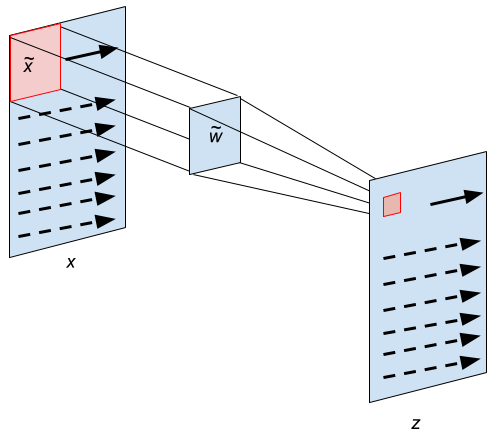
\includegraphics[width=.6\linewidth]{figuras/convwa.png}
	\end{center}
	\small No passo $i,j$, cada operador de projeção $\tilde{\mathbf{w}}$ define um campo de atuação $\tilde{\mathbf{x}}$. Para o canal $\mathbf{z}$, $z_{i,j} = \tilde{\mathbf{w}} \cdot \tilde{\mathbf{x}}$. O produto interno é realizado transformando $\tilde{\mathbf{w}}$ em um vetor linha e $\tilde{\mathbf{x}}$ em um vetor coluna. (Fonte: elaborado pelo autor.)
	\label{convw}
\end{figure}

Como visto, a operação de convolução atua mapeando uma região (do tamanho do núcleo) no canal de entrada em um único pixel no canal de saída. Dada a propriedade de localidade, essas representações podem adicionar muita redundância de informação no canal de saída. Uma forma de contornar o problema é adicionando uma operação de agrupamento (em inglês \textit{pooling}) após as ativações da camada. Uma forma simples de realizar um agrupamento é aplicar um mapa entre um conjunto de pixels de entrada em apenas um pixel de saída, reduzindo o tamanho da representação e forçando a rede a encontrar representações mais eficientes entre os níveis de abstração. Escolhas usuais são a média, o valor máximo (\textit{maxpooling}) ou uma posição fixa das ativações de entrada. As operações de agrupamento podem ser vistas como um tipo especial de convolução (possivelmente não linear) com parâmetros fixos. De fato, uma forma eficiente de implementar agrupamento com um valor fixo é escolher um passo maior que $1$ na operação de convolução.

Camadas de convolução são inspiradas na interpretação vigente do funcionamento do córtex visual de mamíferos. Diferentes camadas hierárquicas são sensíveis à níveis distintos de abstração na representação de imagens: as iniciais apreendem informações de traços simples, posteriormente composições de traços, formas geométricas, objetos complexos e assim por diante. De fato, estudos mais detalhados das projeções hierárquicas aprendidas após o treino por redes convolucionais profundas mostraram similaridades com o seu análogo biológico \cite{lee2008sparse} e crescentes níveis de abstração na representação das imagens \cite{Gatys2015, gatys2016image}, iniciando com traços simples e texturas nas camadas iniciais e culminando em representações abstratas para objetos nas finais.

Frisamos que esta não é uma lista exaustiva dos diferentes tipos de camada que podem ser encontrados na literatura. Não listadas aqui, mas que merecem destaque, podemos citar redes de capsula \cite{sabour2017dynamic}, que desempenham operações de convolução e posterior alinhamento das ativações dos filtros, e redes recorrentes (e suas variações), que adicionam correlação temporal entre os exemplos através de mecanismos de memória. Uma revisão histórica da evolução dessas camadas pode ser encontrado em \cite{jurgenReview2015}. Para uma descrição mais detalhada das arquiteturas descritas nesse capítulo, incluindo limitações, aplicabilidade e detalhes técnicos, ver \cite{Goodfellow-et-al-2016}.

\section{Aprendizado}\label{sec:aprendizado}

Definida a arquitetura da rede neural, isto é, a sequencia das camadas e respectivas funções de ativação, procedemos para o \textit{treino} da rede, que consiste em encontrar os parâmetros ótimos $\\mathbf{Theta}^*$ como definido na equação \ref{thetaotimo}. A forma mais ingênua para procurar o valor ótimo seria utilizar o \textit{método do gradiente} (ou método do máximo declive), que consiste em atualizar iterativamente $\mathbf{\Theta}$ na direção contrária à do gradiente da função custo segundo a regra 
\begin{equation}
\mathbf{\Theta} \leftarrow \mathbf{\Theta} - l_r \nabla_{\mathbf{\Theta}} J^{(D)},
\end{equation}
onde $l_r$ é o \textit{hiper-parâmetro de aprendizado} ou taxa de aprendizado, $D$ o conjunto onde a atualização é realizada e $\nabla_{\mathbf{\Theta}}$ o operador gradiente com respeito aos parâmetros $\mathbf{\Theta}$. A evolução de $\mathbf{\Theta}$ ao longo do treino é referida como \textit{dinâmica do aprendizado}.

O método do gradiente nos garante que, uma vez atingido o mínimo global, o gradiente da função custo é nulo ($\nabla_{\mathbf{\Theta}} J^{(D)} = 0$), e nenhuma atualização posterior se fará necessária. Entretanto, não nos é garantido o recíproco: uma vez que $\nabla_{\mathbf{\Theta}} J^{(D)} = 0$, não podemos afirmar se encontramos um mínimo local, um ponto de sela ou até mesmo um ponto de máximo. Também não é garantido se eventualmente um ponto de gradiente nulo será encontrado. Adicionalmente, a escolha do hiper-parâmetro $l_r$ e do conjunto de atualização $D$ não são especificados pelo método.

Quanto à escolha do conjunto de atualização, podemos escolher dentre atualizar os parâmetros para cada exemplo, para um subconjunto ou para todos os exemplos disponíveis por vez. No primeiro caso, conhecido como \textit{gradiente estocástico}, temos a vantagem de atualizar $\mathbf{\Theta}$ sempre que a rede é exposta à um exemplo, o que poderia levar a uma convergência mais rápida. Essa escolha é comumente referida como aprendizado \textit{online}. Entretanto, as flutuações estatísticas de cada exemplo podem gerar uma condição de difícil convergência, com o gradiente da função custo mudando drasticamente de direção a cada atualização. No outro extremo, conhecido como \textit{gradiente em lote}, $D$ constitui todo o conjunto disponível de treino. Nessa escolha, o gradiente calculado para cada exemplo é acumulado e a atualização é feita pela média dos gradientes em todos os exemplos de treino. Apesar da vantagem da estabilidade estatística, corremos dois riscos: média sobre o conjunto de treino pode anular ou diminuir particularidades de subconjuntos específicos ou podemos demorar demais para atualizar $\mathbf{\Theta}$, o que torna o aprendizado mais lento. Uma terceira opção consiste em juntar o melhor das duas escolhas anteriores: promover a atualização dos parâmetros à cada $N_B$ exemplos. Tal técnica é denominada atualização em mini-lote ou \textit{gradiente em mini-lote} e foi a técnica escolhida no presente trabalho.  

Quanto à escolha de $l_r$ temos que buscar um compromisso entre dois extremos. Valores pequenos produzem dinâmicas lentas, onde as atualizações do parâmetros são pequenas e o tempo de treino se estende por diversas iterações. Em alguns casos, a dinâmica pode estagnar em regiões onde $\nabla_{\mathbf{\Theta}} J^{(D)}$ é pequeno mas o valor do custo ainda é alto. No outro extremo, temos uma dinâmica mais rápida, porem mais instável. Pontos de mínimo podem ser completamente ignorados (fenômeno referido como \textit{overshoot}) e a função de erro tende a exibir flutuações que dificultam a convergência. Para valores extremamente altos, a dinâmica pode superestimar os erros cometidos e/ou amplificar demais as flutuações, fazendo o valor do custo aumentar ao invés de diminuir. Uma maneira de contornar o problema é utilizar uma abordagem adaptativa. Uma solução simples é diminuir o valor da taxa de aprendizado ao longo do treino, sendo decaimento linear ou exponencial duas escolhas bastante comuns. Dessa forma, temos um balanço entre rápido aprendizado no início da dinâmica e maior estabilidade próximo ao fim. Outras técnicas incluem estabelecer regras de atualização baseadas no gradiente da função de custo e no momento (taxa de atualização do gradiente). A descrição detalhada dessas técnicas fogem ao escopo deste trabalho. Nos experimentos utilizamos a técnica conhecida como Estimativa Adaptativa do Momento (em inglês, \textit{Adaptive Moment Estimation}), também referida como Adam \cite{adam_op} que foi especialmente desenvolvida para atualizações em mini-lote e utiliza o momento dos gradientes do custo para estabilizar o aprendizado e decaimento da taxa de treino. Um exemplo esquemático de uma dinâmica lenta ($l_r$ pequeno) e rápida ($l_r$ grande) pode ser vista na figura \ref{convergence}.

\begin{figure}[ht]
	\caption{Exemplo de comportamento característico da função de custo.}
	\begin{center}
	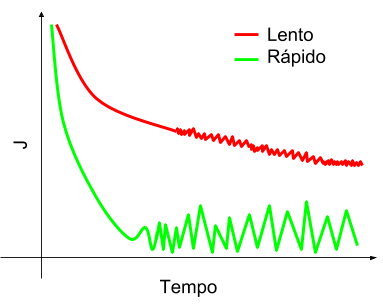
\includegraphics[width=.6\linewidth]{figuras/convergence.png}
	\end{center}
	\small Em vermelho o aprendizado é lento e apresenta flutuações menores. Em verde o custo decai rapidamente, mas apresenta flutuações mais drásticas. (Fonte: elaborado pelo autor.)
	\label{convergence}
\end{figure}


Para redes compostas por várias camadas, como descrito na equação \ref{fcamadas}, a atualização dos parâmetros torna-se complicada e potencialmente suscetível a erros numéricos. Uma forma eficiente de contornar o problema é utilizar a técnica de propagação reversa (em inglês \textit{back-propagation}). Nesta técnica, a computação realizada pela rede é mapeada em um grafo, sendo cada operação realizada na computação expresso como um nó e o fluxo de dados entre duas operações representado por uma aresta direcionada. Durante a fase direta (\textit{feed-foward}) a computação é executada nó-a-nó e os resultados parciais de cada operação armazenados. Durante a fase reversa, as arestas são invertidas e o erro propagado entre os vértices do grafo reverso utilizando-se os valores previamente armazenados e a regra da cadeia para expressar a dependência entre os erros. Durante essa etapa, cada nó que possui um parâmetro a ser aprendido é atualizado. Ver \cite{jurgenReview2015} para uma revisão do método.


\section{Regularização}

Como visto da seção \ref{sec:aprendizado}, durante a evolução da dinâmica de aprendizado, os parâmetros da rede evoluem de forma a reduzir o valor esperado da função de custo no conjunto de treino. Entretanto, diminuir o erro nos exemplos vistos não garante que o modelo apresentará a mesma qualidade em novos elementos ausentes durante essa fase. De forma mais precisa, seja $U$ o conjunto de todos elemento-rótulo possíveis, tipicamente temos a disposição um subconjunto $D \subset U$ para otimizar a rede, e utilizamos $J^{(D)}$ como um estimador estatístico para $J^{(U)}$, isto é, supondo que $D$ tenha sido formado por instâncias aleatórias de $U$, teremos $J^{(D)} \rightarrow J^{(U)}$ quando $|D| \rightarrow |U|$. Tipicamente, entretanto, temos a situação em que $|D| \lll |U|$. Como o modelo foi otimizado neste subconjunto, o valor esperado da função custo em $D$ se torna um estimador enviesado para o erro esperado em exemplos não vistos. Uma maneira simples e eficiente de estimar a capacidade de generalização modelo é criar a cobertura exata $(D_{tr}, D_{val})$ para $D$, treinar o modelo em $D_{tr}$ e acessar sua qualidade em $D_{val}$. Esta técnica é conhecida como \textit{hold-out}, e $J^{(D_{val})}$ uma estimativa para o poder de generalização do modelo \cite{friedman2001elements}.

Um outro problema recorrente no treino de modelos de aprendizado de máquina é a adaptação do modelo ao conjunto de treino. Em um extremo, modelos de baixa expressividade podem não conseguir capturar a complexidade das relações exemplo-rótulo. Esse fenômeno é conhecido como \textit{underfitting}. No outro limite, a medida que aumentamos a expressividade (mais camadas, mais projeções, etc.), aumenta também capacidade de apreender relações mais complexas entre exemplos e rótulos. Entretanto, modelos com maior expressividade tendem a ser mais propensos a '\textit{decorar}' exceções e superestimar particularidades do conjunto de treino. Tal fenômeno é conhecido como coadaptação ou \textit{overfitting}. Outra situação em que podemos incorrer em \textit{overfitting} é quando o modelo é excessivamente exposto aos mesmos exemplos durante uma seção de treino. O \textit{underfitting} pode ser detectado diretamente da qualidade do modelo em $D_{tr}$, quando seu desempenho se mostra aquém do esperado. O segundo pode ser estimado utilizando a decomposição \textit{viés-variância} da estimativa do erro, onde entendemos que parte do erro cometido é devido a baixa expressividade e parte por superestimar particularidades do conjunto de treino. Para tal, a qualidade do modelo em $D_{tr}$ e sua capacidade de generalização (estimada em $D_{val}$) são comparadas e a diferença entre as duas servem para estimar a relação entre viés e variância. Um exemplo ilustrativo do comportamento do erro nesses dois conjuntos pode ser visto na figura \ref{overfit}.

\begin{figure}[ht]
	\caption{Exemplo ilustrativo de \textit{overfitting} e \textit{underfitting}.}
 	\begin{center}
	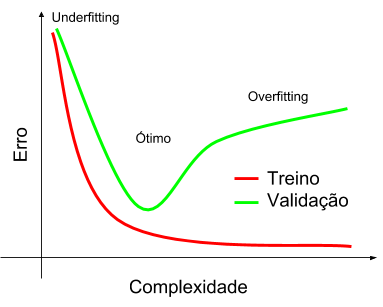
\includegraphics[width=.6\linewidth]{figuras/overfitting.png}
	\end{center}
	\small Em verde vemos que o erro estimado no conjunto de treino se comporta como uma função decrescente da complexidade do modelo. Em vermelho, o erro estimado o conjunto de validação mostra que existe um valor ótimo para o poder de generalização. Fixada a complexidade do modelo, experimenta-se um comportamento similar quando aumentamos a exposição aos exemplos no conjunto de treino. (Fonte: elaborado pelo autor.)
	\label{overfit}
\end{figure}

Para minimizar o efeito de coadaptação dos parâmetros, podemos impor condições extras durante o processo de aprendizado. Uma das condições mais usuais é aplicar ao vetor de parâmetros $\mathbf{\Theta}$ alguma restrição. Podemos, por exemplo, adicionar à função custo um termo proporcional à norma do vetor $\mathbf{\Theta}$, na forma
\begin{equation}
\tilde{J} = J + \lambda \left| \mathbf{\Theta} \right|_p,
\end{equation}
onde $\tilde{J}$ é o custo utilizado durante a minimização, $\left| \mathbf{\Theta} \right|_p = \sqrt[p]{\mathbf{\Theta}^p}$ é a norma $p$ e $\lambda$ o hiper-parâmetro de regularização ou constante de normalização. Desta forma penalizamos parâmetros que '\textit{aprendam}' demais uma determinada característica. Apesar de efetivo, o uso de regularização baseado em normas adiciona dois novos hiper-parâmetros: a constante de normalização e o tipo de norma que devemos usar. Outra forma de regularização comum na literatura é o \textit{dropout} \cite{hinton2012improving}. Nesta técnica, a saída $i$ de uma camada é removida da computação (atribuída o valor zero) com uma probabilidade $p$, hiper-parâmetro da técnica. Intuitivamente, o uso do \textit{dropout} durante o treino força a rede a encontrar representações redundantes e mais robustas à detalhes, dado que a cada nova iteração uma característica aprendida anteriormente pode estar ausente.

\section{Redes Neurais e CAPTCHAs}

Como visto na secção \ref{sec:captchatexto}, CAPTCHAs de texto podem ser vistos como um problema de extração de texto em imagens, sendo assim uma generalização para o problema de OCR e um subproblema de localização de texto em imagens (identificar, se existir, a localização de todos os textos em uma imagem). É preciso ressaltar, entretanto, que nesses HIPs as imagens são especialmente desenvolvidas para serem de difícil solução para computadores e preferencialmente fáceis para seres humanos. Assim, algoritmos usuais de OCR tendem a demonstrar baixo desempenho na solução desses desafios. Vamos separar as abordagens para o problema em dois grandes grupos: abordagens \textit{informadas} e não \textit{informadas}.

Em abordagens informadas o autor do ataque estuda os efeitos e o alfabeto utilizado na composição do desafio e confecciona um pipeline para preprocessamento e segmentação dos caracteres componentes do token. Esta etapa envolve o uso de heurísticas e é extremamente dependente da regularidade das imagens\footnote{Isso é tipicamente verdade quando a imagem é gerada automaticamente por um computador. Neste caso, técnicas de engenharia reversa podem guiar o desenvolvimento de heurísticas.} e da habilidade do atacante para que bons resultados sejam alcançados. Após a segmentação, o desafio se resume à reconhecer corretamente cada símbolo. Um dos trabalhos pioneiros na quebra de CAPTCHAs de texto foi conduzido por \cite{lectures2005HIP} e utiliza essa abordagem. Inicialmente as imagens foram preprocessadas e segmentadas. Para o reconhecimento foram usadas redes convolucionais de duas camadas, alcançando acurácias entre $10\%$ e $50\%$ (fortemente dependente da qualidade do preprocessamento). Bursztein \textit{et al.} formalizaram ainda mais o pipeline de processamento, lançando a ferramenta \textit{Decaptcha} \cite{bursztein2011text}, que permite explorar e testar etapas do processo de quebra especificando-se técnicas de preprocessamento, segmentação, pos-segmentação, reconhecimento e aprimoramento pós reconhecimento. Com o auxilio dessa ferramenta, os autores relataram modelos com acurácias mais baixas em trono de $20\%$, chegando $100\%$ de acertos em desafios mais simples. Entretanto, como sugerido pelos próprios autores, na fase de reconhecimento a ferramente utiliza algoritmos com baixo poder de expressividade (k-vizinhos mais próximos e máquinas de vetores de suporte) se comparados com técnicas mais atuais. Se olharmos apenas para o desafio pós segmentação, a extração de texto de CAPTCHAs se resume a um problema de reconhecimento de caracteres, e nesse campo o estado da arte é dominado por redes neurais. De fato, no repositório do MNIST\footnote{O MNIST (Modified National Institute of Standards and Technology database) é um repositório aberto contendo 70000 imagens de dígitos escritos à mão e usualmente usado como benchmark para técnicas de OCR. A tarefa consiste em reconhecer corretamente o número codificado na imagem. No sítio do repositório existe uma tabela comparativa da precisão de diversos estudos publicados utilizando-se diferentes técnicas ao longo dos anos.} \cite{yann1998mnist}, por exemplo, redes convolucionais pontuam entre as melhores taxas de acerto, sendo o melhor modelo registrado o desenvolvido por {Cire{\c s}an} \textit{et al.}, que alcançou $99.77\%$ de acerto e é baseado na média do voto de 35 redes convolucionais independentes \cite{ciresan2012column}. Para CAPTCHAs de texto formados por imagens reais, as diversas condições de aquisição (iluminação, ângulo, escala, etc.) degradam as vantagens de um pipeline único de preprocessamento. Mesmo neste caso, redes neurais ainda são capazes de demonstrar bom desempenho. Netzer \textit{et al.} propuseram o repositório SVHN\footnote{SVHN (Street View House Numbers), composto por mais de 600000 fotos de fachadas de construções contendo números. O desafio consistem em reconhecer corretamente os algarismos codificados na imagem. O repositório possui dois formatos para os mesmas imagens: a) Caracteres segmentados; e b) Apenas a região contendo os números.} como benchmark para esse tipo de desafio \cite{netzer2011reading}. Partindo das imagens já segmentadas, os autores foram capazes de obter precisões em torno de $90\%$ utilizando-se abordagens não supervisionadas de redes neurais. O resultado foi posteriormente refinado utilizando-se redes convolucionais profundas e treino supervisionado, alcançando $94.5\%$ de precisão \cite{sermanet2012convolutional}.

Quanto às abordagens não informadas, o modelo deve aprender de forma autônoma como localizar, segmentar e reconhecer os caracteres em uma imagem, minimizando a interferência direta humana. Entretanto, inferir esse nível de abstração apenas baseado em exemplos pode requerer quantidades massivas de dados anotados. Utilizando uma abordagem não informada, Goodfellow \textit{et al.} foram capazes de obter $99.8\%$ de acerto nos textos da primeira versão do reCAPTCHA \cite{captcha_break_2013}. Os autores ainda conduziram um estudo no repositório SVHN, obtendo acertos de $97.84\%$ por caractere e $96\%$ para o token completo. Entretanto, a base de treino utilizada era formada por 600 mil imagens para o SVHN (toda a base de teino) e mais de um milhão de imagens para o reCaptcha. Mais recentemente, foi investigada uma alternativa para diminuir volume de dados necessário para esse tipo de abordagem através de uma nova arquitetura denominada Redes Corticais Recorrentes (do inglês, Recurrent Cortical Network) \cite{captcha_break_2017}. Utilizando esta nova arquitetura, os autores do estudo relataram uma alta eficiência de dados, obtendo resultados satisfatórios com algumas milhares ou até mesmo centenas de exemplos. O diferencial dessa arquitetura são conexões extras adicionadas entre as camadas que permite um fluxo mais complexo da informação. Aplicada à quebra de CAPTCHA, os autores treinaram esse tipo de rede em imagens contendo diferentes fontes tipográficas para o mesmo alfabeto. Durante a validação, a arquitetura mostrou capacidade de generalizar e abstrair as transformações aplicadas em CAPTCHAs sintéticos, sendo capaz de reconhecer os símbolos mesmo após as deformações. Um ponto negativo, entretanto, é o tempo de treino dessa nova arquitetura. As mensagens trocadas entres as camadas e o algoritmo proposto para supressão de característica limitam a capacidade de paralelização e tornam a execução mais lenta. De fato, há uma nota no repositório dos autores informando que o treino em 1000 imagens do desafio MNIST (onde o algoritmo se aproxima do estado da arte nesse desafio) pode levar horas em múltiplas CPUs\footnote{Fonte: \url{https://github.com/vicariousinc/science_rcn}. Acesso em: 23/06/2018.}. Adicionalmente, os autores alegam que fizeram ajustes nos filtros convolucionais e nas fontes de treino para cada aplicação, o que pode ser interpretado com uma forma de adicionar viés ao modelo (algo como uma abordagem semi-informada). Em um estudo similar ao nosso, Pinto alcançou $76,6\%$ de precisão na quebra CAPTCHAs de texto utilizando redes neurais profundas. Contudo, foram necessários uma base de treino com 180 mil imagens e placas de processamento gráfico de última geração, sendo o treino realizado em sistemas de computação sob demanda \cite{otaro}. Sendo este o trabalho mais recente diretamente relacionado ao nosso encontrado na literatura, o definimos como trabalho de referência para comparações com os resultados obtidos em nosso trabalho.

Diante disso, apesar da qualidade dos resultados encontrados na literatura, os requisitos desses sistemas os tornam proibitivos para serem treinados em computadores comuns. Na tabela \ref{tableredes} apresentamos um breve comparativo dos requisitos de alguns dos estudos selecionados. Essas restrições limitam o acesso dessa tecnologia à ambientes com menor poder de processamento ou restrições orçamentárias. É particularmente proibitivo para o estudante médio brasileiro, o que pode gerar uma defasagem de aprendizado tecnológico, e para pequenas empresas experimentarem soluções inovadoras baseadas nessas descobertas. Assim, o objetivo deste trabalho é propor um abordagem construtiva para a experimentação de redes neurais profundas em computadores comuns focada no problema de \textbf{quebra não informada de CAPTCHAs de texto}. Pretendemos mostrar que é possível alcançar resultados próximos ao estado da arte a partir da investigação cautelosa do comportamento dos modelos durante a dinâmica de treino, com bases de treinos menores e arquiteturas mais simples. 


\begin{table}[ht]
\begin{center}
	\caption{Comparação entre os requisitos dos modelos encontrados na literatura.}
	\begin{tabular}{ c | >{\centering\arraybackslash}m{7cm}  }
		Referência & Limitação  \\ %\hline
		\hline \hline  
		Netzer \textit{et al.}     \cite{netzer2011reading}         &  600 mil imagens, 500 filtros convolucionais 8x8.  \\ \hline
		Sermanet \textit{et al.}   \cite{sermanet2012convolutional} &  16 filtros 5x5, 512 filtros 7x7, 2 camadas densas de 4000 entradas. \\ \hline
		Goodfellow \textit{et al.} \cite{captcha_break_2013}        &  De 9 a 11 camadas convolucionais (8-192 filtros), camada densa com mais de 3 mil entradas, mais de 500 mil exemplos.   \\ \hline
		Pinto \cite{otaro}											& 180 mil exemplos, quatro camadas convolucionais com 64, 128, 256 e 512 canais, duas camadas densas com mais de 4000 entradas, totalizando mais de $6 \, 10^{7}$ parâmetros.\\ \hline
		Dileep \textit{et al.} \cite{captcha_break_2017}			& Treinameto de difícil paralelização. Muitas horas de treino para alcançar resultados satisfatórios. Necessidade de acompanhamento por humanos.\\ \hline
\end{tabular}
	\label{tableredes}
\end{center}
\end{table}
